% Mirror: https://github.com/SIGma-UIUC/presentation-format
% --------------------------------------------------------------------
% This is a simple Beamer document that uses beamerthemesigma.sty
% Reading the comments should help you create a presentation even if
% you've never used Beamer before.
% --------------------------------------------------------------------

% Set our document class to Beamer
\documentclass[aspectratio=169]{beamer}
% \documentclass[aspectratio=169, handout]{beamer}
% Add handout option to ignore pauses

% From Jeff E
\usepackage{algo}
% Some more macros
\usepackage{sigmastyle}


% Set a title
\title{Quantum Complexity Theory}

% Set a subtitle if you desire
%\subtitle{[TAOCP 5 8.9.10.11]}

% Whoever worked on the presentation:
\author{Eyad Loutfi}

% Date looks ugly, so leave blank
\date{"My contention is the following: Quantum mechanics is what you would inevitably come up with if you started from probability theory, and then said, let's try to generalize it so that the numbers we used to call `probabilities' can be negative numbers. As such, the theory could have been invented by mathematicians in the 19th century without any input from experiment. It wasn't, but it could have been." \\ - Scott Aaronson}

% An institute name, if you're so inclined
% \institute{University of Illinois Urbana-Champaign}

% Use the SIGma theme for this Beamer presentation
\usetheme{sigma}
% --------------------------------------------------------------------

% Begin document
\begin{document}

% Beamer calls each slide a "frame", defined within the environment:
% \begin{frame}
%   <frame content here>
% \end{frame}

% This frame is just the title.
\begin{frame}
\titlepage
\end{frame}

\section{Basics of Complexity}
% Section pages can be printed thus:
\frame{\sectionpage}

\begin{frame}{Turing Machines}
  
  \begin{itemize}
    \item First we need to introduce our model of computation. The classic model of computation is the \emph{Turing machine}. \pause
    \item TM's are defined over a finite alphabet, have an infinite tape that has the input at the start of it, a read head with internal state that starts at the start of the tape and can write or move left or right all according to some finite instructions (represented as a transition function based on the head's state and character in the cell it's over). 
  \end{itemize}
  \begin{center}
    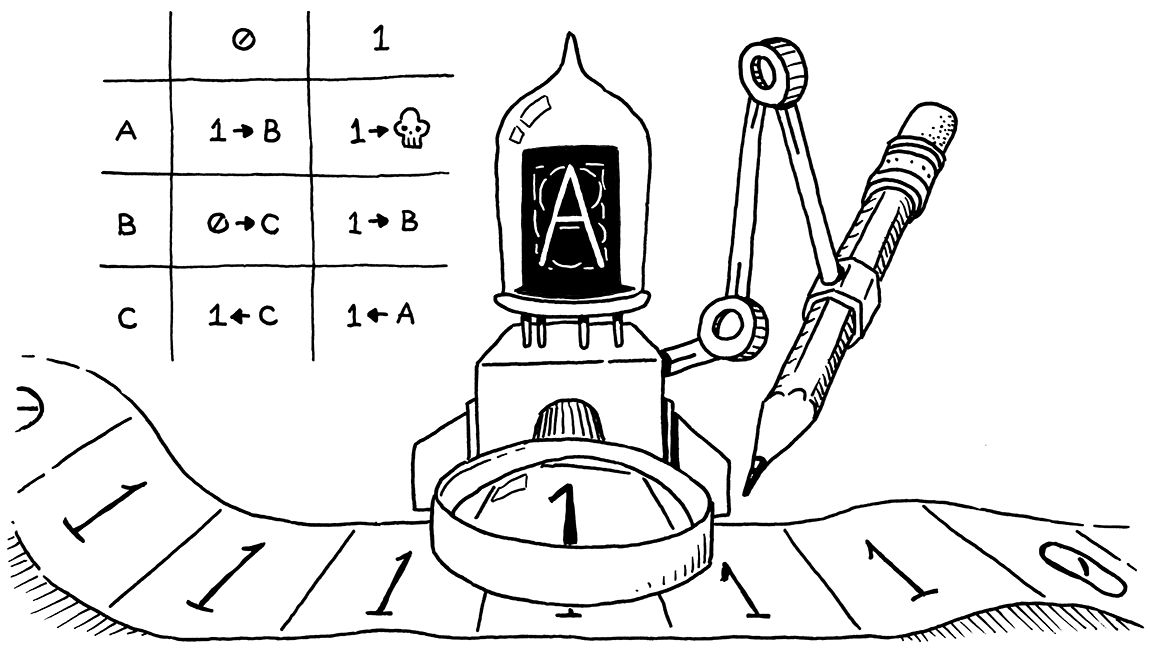
\includegraphics[width=0.5\textwidth, height=0.5\textheight, keepaspectratio]{Turing_pic.png}
  \end{center}
\end{frame}

\begin{frame}{Turing Machines}
  
  \begin{itemize}
    \item A more intuitive way to think about TM's - and that makes it clear why this is a very natural definition to come up with if you live in a time before computers - is to consider a model with the following features: \pause
    \begin{itemize} 
        \item The world as an idealized grid \pause
        \item An idealized mathematician who can only move one cell at a time \pause
        \item Can read and write one symbol at a time (alternatively, can simply change the symbols/"alphabet" to represent words, doesn't matter so long as there's only a finite number of choices). \pause
    \end{itemize} 
    \item All choices one can make is finite - implicitly a function or "response" of a finite number of states of ourselves and our surrounding environment. Note these "finite instructions" can still yield unbounded behavior. We're allowing behavior to go on forever, whereas in real life us and computers have finite lives.
  \end{itemize}
\end{frame}

\begin{frame}{Turing Machines}
  
  \begin{itemize} 
    \item While this might seem extremely broad and philosophical - and not specifically the same: That's the point! While we won't prove it, the Turing Machine model is very robust, you can change numerous specifics without effecting most results in the field. \pause
    \item i.e. changing the number of tapes or the dimension of the tape does not change computability at all. \pause
    \item Moreover if we're trying to study problems based on intrinsic difficulty, complexity theorists often classify problems broadly on whether they require polynomial or exponential time. These changes to a TM can provably gain at most only a polynomial speedup, so it does not make a difference. This all points in the direction of the Turing machine being the "right model."
  \end{itemize}
\end{frame}

\begin{frame}{Computability}
  
  \begin{itemize}
    \item Specifically, the \emph{Church Turing} thesis states that anything that can be "computed" can be done by a Turing machine. While this is not a formal statement, and therefore not the type that can even be proved, hopefully you've seen why intuitively it feels self evident. \pause
    \item Note that once we fix the exact TM model, like programs they end up being defined by precise descriptions, so in a sense they are strings themselves! \pause
    \item One can devise an encoding scheme of all programs -- many such encodings exist, could use all binary strings or all ASCII strings, etc.
  \end{itemize}
\end{frame}

\begin{frame}{Computability}
  
  \begin{itemize}
    \item More importantly, the encoding is done in such a way that a program can recognize it -- such that we can define a program to simulate the behavior of a machine as a result of parsing the encoding. \pause
    \item This means we can define a program to be able to simulate any other program -- a very important result! \pause
    \item Other important definitions: A set is ``recursively enumerable,'' or RE if there exists a program that can give a ``yes'' answer to any string in the set. A set is ``computable'' or ``decidable" if a program like that exists that also gives a ``no'' answer for any string not in the set. \pause
    \item These properties are not guaranteed in general due to possibility of infinite looping.
  \end{itemize}
\end{frame}

\begin{frame}{Complexity Basics}
  
  \begin{itemize}
    \item Computability and complexity theory are the study of the fundamental limitations of computation - namely computability in the former, and time and space requirements in the latter. \pause 
    \item Specifically we will often study these in the context of \emph{decision problems}, problems phrased as "yes" or "no" answers to whether an input is in a set. Typically, the decision problem and the corresponding set - or "language" that defines it are used interchangeably in the language of theoretical computer science. 
  \end{itemize}
\end{frame}

\begin{frame}
  % Alternate syntax for frame titles
  \frametitle{Uncomputability}
  % Frames can have subtitles:
  % Some frame content:
  \item We can further prove not all decision problems are computable. 
  \begin{thrm}
    The halting problem is undecidable. That is - the set of all pairs of encodings of Turing Machines with inputs (so an arbitrary $\langle M, x\rangle$), such that that respective Turing machine halts on that input - is an uncomputable set. 
  \end{thrm}
  \pause
  \begin{pf}
    \begin{enumerate}
        \item Suppose not. That is $\exists$ TM M that decides this set. \pause
        \item We can create a new machine $M'$ that simulates $M$ on the input to $M'$, such that if the input is an encoding of a machine that halts, we program $M'$ to loop forever, while if it's a machine that loops forever, we program $M'$ to halt. \pause
        \item Now if we give $M'$ the input $\langle M', \langle M' \rangle \rangle$, this implies $M'$ halts on $\langle M' \rangle \Leftrightarrow$ $M'$ loops forever on it - a contradiction.
    \end{enumerate}
  \end{pf}
\end{frame}

\begin{frame}{Diagonalization}
  
  \begin{itemize}
    \item This technique of creating a contradiction through self reference, called diagonalization will be seen again. \pause
    \item Often involves assuming some self referential structure with a property is true, then constructing a similar structure that fulfills the opposite of that property, asking a carefully constructed question about itself that will lead to contradiction. \pause
    \item Diagonalization was the \emph{cornerstone} of basically all early results in logic, set theory, computability, and complexity theory during the late 19th and first half of the 20th century. 
  \end{itemize}
\end{frame}

\begin{frame}{Diagonalization - Other Examples}
  \begin{itemize}
    \begin{itemize}
        \item "This sentence is a lie." Is this sentence the truth or a lie? \pause
        \item Descartes - "I think therefore I am." Suppose your thoughts do not exist. Now ask "does the thought of `your thoughts do not exist'" exist? \pause 
        \item Russell - Suppose the set of all sets that do not contain themselves exists. Now ask, "does this set contain itself"? \pause
        \item Godel - Consider the guaranteed to exist Godel sentence of any axiom system F that contains even just basic arithmetic, which is the statement $G \Leftrightarrow$ "$F$ does not prove $G$". Now ask, "can $F$ prove $G$"?
    \end{itemize}
  \end{itemize}
  \begin{flushright}
    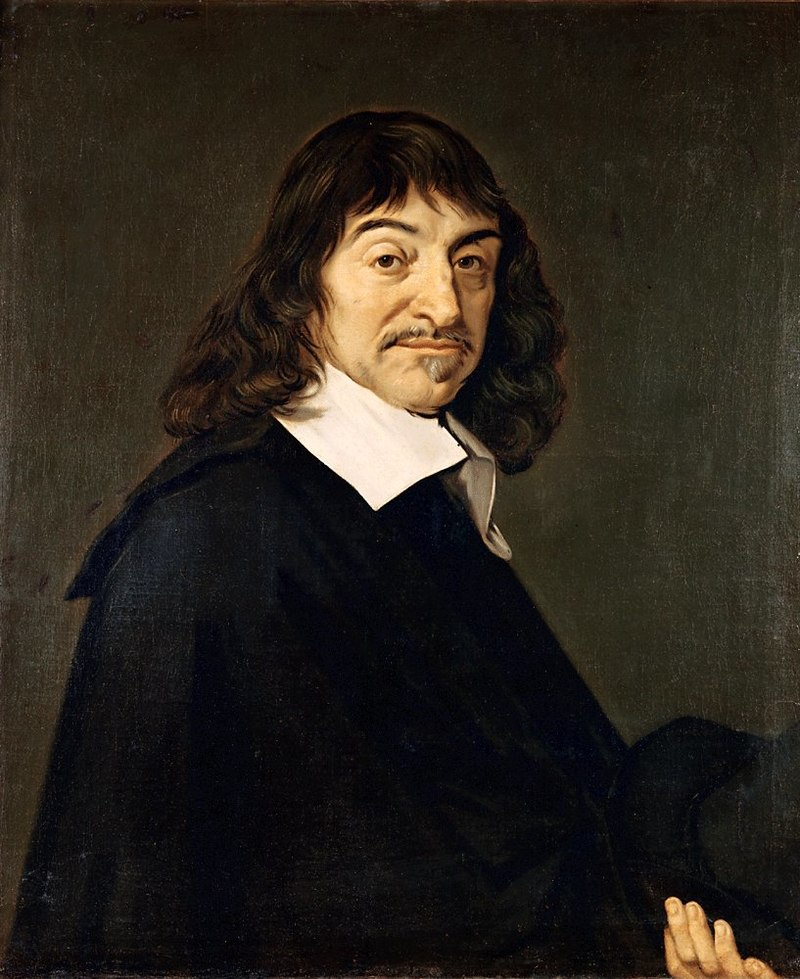
\includegraphics[width=0.3\textwidth, height=0.3\textheight, keepaspectratio]{Descartes.jpg}
  \end{flushright}
\end{frame}

\begin{frame}{Diagonalization - Other Examples}
  \begin{itemize}
    \item Cantor - Suppose the real numbers between $0$ and $1$ can be listed on a list enumerated by the natural numbers. Is the real number in $(0, 1)$ that's $i$th digit is different from the $i$th digit of the $i$th real number on that list, in that list? (This is why it's "diagonal").
  \end{itemize}
  \begin{center}
    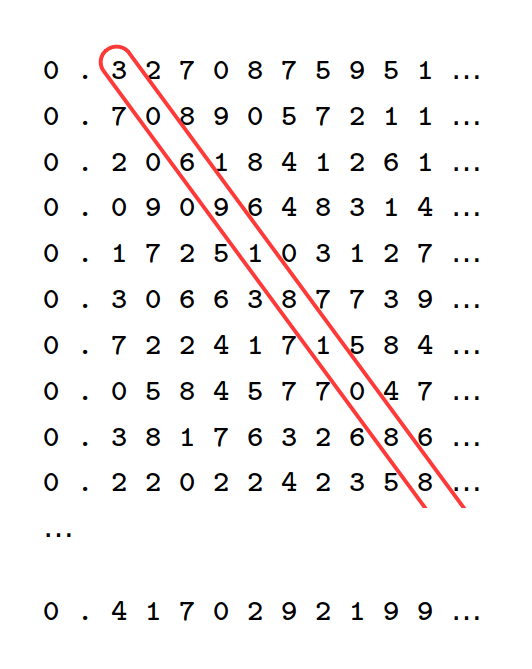
\includegraphics[width=0.6\textwidth, height=0.6\textheight, keepaspectratio]{uncountable.png}
  \end{center}
\end{frame}

\begin{frame}{Complexity Basics}
  
  \begin{itemize}
    \item P is the class of all computable sets for which a Turing machine exists that gives a "yes" or "no" answer to membership with a polynomial number of steps relative to the input size. \pause
    \item NP is the class of all computable sets for which a Turing machine exists that, while not required to have such a polynomial runtime, there will exist some other Turing Machine called a "verifier." \pause
    \item The verifier takes in a second input in addition to the regular input, such that for all strings $x$ in the set, there exists a string $s$ where $|s| = poly(|x|)$ such that $s$ being in the second input will cause the Turing machine to accept in polynomial time. We therefore say that NP is the class of problems that have polynomial verification for "yes" answers.
  \end{itemize}
\end{frame}

\begin{frame}{Complexity Basics}
  
  \begin{itemize}
    \item This "special string" is often called a "witness" or "certificate" and can be thought of as a "proof" for membership of the regular input, specifically a polynomial sized proof. \pause
    \item It may be strange to connect proofs to computability, however all methods for doing proofs that we know of are in fact via computable inference rules - rules that can be programmed into a Turing Machine. Therefore provability "under the hood" is really just knowledge that's computable. \pause
    \item P is trivially in NP - can simply choose corresponding polynomial time Turing Machine for a set in $P$ and have any string accepted as the second input for the verifier. \pause
    \item The other direction however, if $NP \subseteq P$ is unknown and known to be one of the biggest open problems in Math and Computer Science.
  \end{itemize}
\end{frame}


\begin{frame}{Complexity Basics}
  
  \begin{itemize}
    \item In general the class \emph{DTIME(T(n))} is the set of all problems that can be solved by a Turing machine with time $T(n)$ relative to input size, and likewise \emph{DSPACE(T(n))} is the same but for the corresponding space requirement instead of the time requirement. \pause
    \item For any complexity class $A$, the class co-$A$ is the set of complements of decision problems in $A$. Namely, this means co-NP is identified by stipulating polynomial time verification for "no" answers rather than "yes" answers. It is also an open problem whether NP $=$ co-NP. \pause
    \item Intuitively most of the canonical NP problems you can think of, Boolean/Circuit satisfiability, Travelling Salesman, etc are problems with which we don't know how to do better than an exponential brute force search looking for a certain solution (or lack thereof), but which you could immediately confirm/"verify" if you actually had that solution.
  \end{itemize}
\end{frame}

\begin{frame}{Complexity Basics - Reductions}
  
  \begin{itemize}
    \item In the context of computability theory, we say a problem $Q$ reduces to $K$, or $Q \leq K$ if solving $K$ enables us to solve $Q$. This is called a \empth{reduction}. \pause
    \item In the context of complexity theory, we say the same only if it enables us to solve $Q$ in polynomial time. While we still call it a reduction, it's a \emph{polynomial time reduction}, because the exact reduction/algorithm that uses our answer to $K$ to solve $Q$ has to run in polynomial time. \pause
    \item For a class $A$, we say a problem is $A$-hard if every problem in $A$ reduces to it. We say it's $A$-complete if it's $A$-hard and also in $A$.
  \end{itemize}
\end{frame}

\begin{frame}{Complexity Basics}
  
  \begin{itemize}
    \item What we think the world looks like (but have yet to prove):
  \end{itemize}
  \begin{center}
    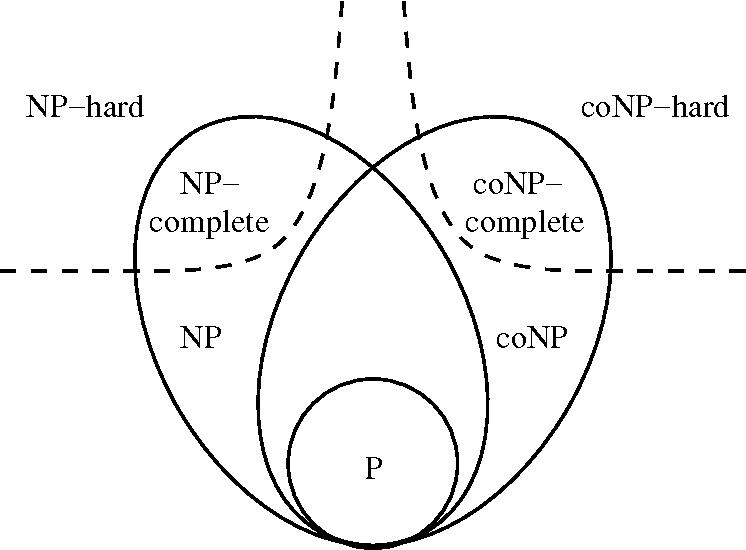
\includegraphics[width=0.6\textwidth, height=0.6\textheight, keepaspectratio]{PNP.png}
  \end{center}
\end{frame}

\begin{frame}{Complexity Basics - Oracles}
  
  \begin{itemize}
    \item We will often also consider computational power with \emph{oracles}. An oracle $O$ for a problem $K$ is a black box we can give our machine access to, such that whenever it gives it an input it instantly outputs the answer to $K$ for that input. \pause
    \item The class $A^B$ is the set of problems that would be in $A$ if we allow Turing machines access to oracles for problems in $B$. \pause
    \item Going back to computability theory, you can actually define an oracle for undecidable problems like the halting problem, and even then there are still other undecidable problems. \pause
    \item Since we can keep giving oracles for those, this yields an infinite tower of classes of undecidable problems that quantifies how undecidable they are - called the arithmetic hierarchy. 
  \end{itemize}
\end{frame}

\begin{frame}{Hierarchy of Complexity}

  \begin{center}
    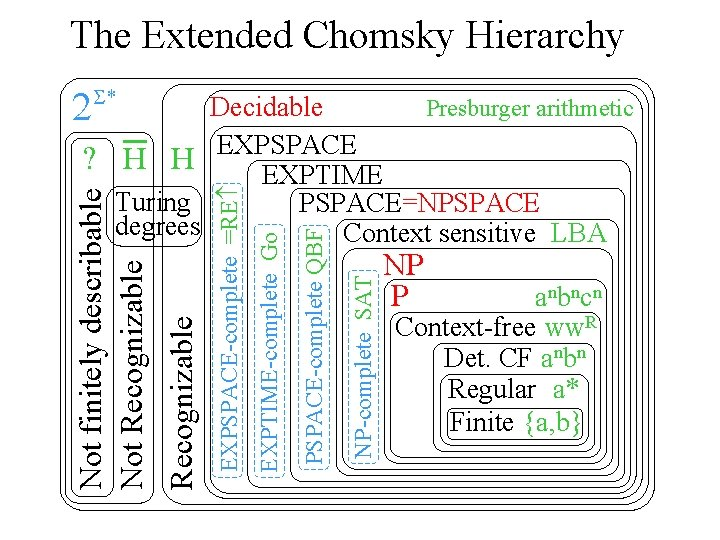
\includegraphics[width=0.9\textwidth, height=0.9\textheight, keepaspectratio]{chomsky.jpg}
  \end{center}
\end{frame}

\begin{frame}{Complexity Basics - Polynomial Hierarchy}
  
  \begin{itemize}
    \item Similar to the Arithmetic Hierarchy, we can apply the same logic of building an infinite tower by successively adding oracles for the previous levels - but this time specifically to the class NP. \pause
    \item What we obtain is called the polynomial hierarchy, however this has a lot more uncertainty regarding it, namely if any of the levels are distinct at all (for instance if P $=$ NP or any two successive levels are the same, the hierarchy above it collapses). 
  \end{itemize}
  \begin{center}
    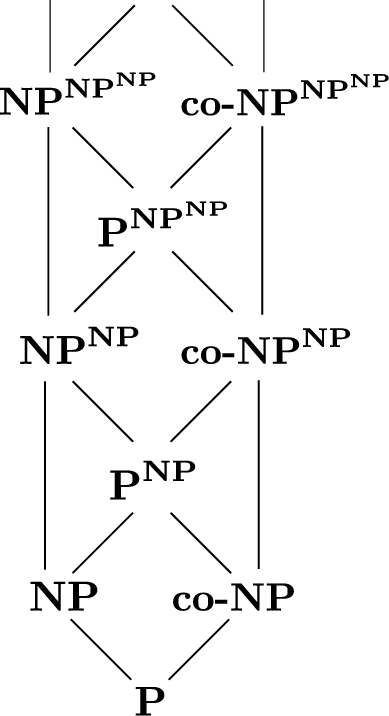
\includegraphics[width=0.4\textwidth, height=0.4\textheight, keepaspectratio]{polynomial hiearchy.png}
  \end{center}
\end{frame}

% Start a section: *sections* (subsections, etc.) are what show up in the TOC.
\section{Quantum Computing}
% Section pages can be printed thus:
\frame{\sectionpage}
% There's a way to automate this, see:
% https://tex.stackexchange.com/questions/178800/creating-sections-each-with-title-pages-in-beamers-slides/178803

\begin{frame}{Qubits}
  \begin{itemize}
    \item A qubit is essentially a unit vector, $\alpha |0\rangle + \beta |1\rangle$, where $\{|0\rangle, |1\rangle\}$ is our standard orthonormal basis, representing the classical bits $0$ and $1$ respectively, and $\alpha, \beta \in \mathbb{C}$. \pause
    \item Whereas a qubit may be equal to one of those bits, in general it's neither, and we refer to it as a \emph{superposition} of those states, until we apply what's called $\emph{measurement}$. \pause
    \item Once we do that, it will be a $0$ with probability $\alpha^2$ and a $1$ with probability $\beta^2$. \pause
    \item Note that the stipulation that it's a unit vector implies $\alpha^2 + \beta^2 = 1$.
  \end{itemize}
\end{frame}

\begin{frame}{Quantum Gates}
  \begin{itemize}
    \item We can further perform logical operations on qubits like we could for classical bits, these "quantum gates" are essentially unitary matrices. \pause
    \item A matrix being unitary means it has an inverse, and namely it's inverse is it's conjugate transpose. \pause
    \item It furthermore has the property that it preserves inner products and norms, so our vector will remain a unit vector. 
  \end{itemize}
\end{frame}

\begin{frame}{Multiple Qubits}
   \begin{center}
    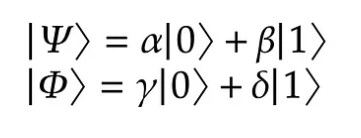
\includegraphics[width=0.4\textwidth, height=0.4\textheight, keepaspectratio]{tensor1.PNG}
  \end{center}
  \begin{itemize}
    \item If we have multiple qubits together like above, we can define it as one state via the tensor product: \pause
  \end{itemize}
  \begin{center}
    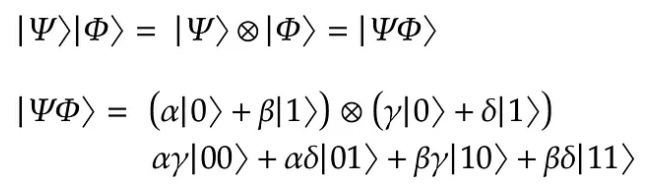
\includegraphics[width=0.6\textwidth, height=0.6\textheight, keepaspectratio]{tensor2.PNG}
  \end{center} \pause
  \begin{itemize}
    \item Note that the sum of the squares of the coefficients is still equal to $1$.
  \end{itemize}
\end{frame}

\begin{frame}{Multiple Qubits Continued}
  \begin{itemize}
    \item In general the state vector of $n$ qubits is expressed as $\sum_{x \in \{0,1\}^n} \alpha_x |x\rangle$ where $\sum_{x \in \{0,1\}^n} \alpha_x^2 = 1$. \pause
    \item While we can apply unitaries/gate operations to a multi qubit system, note that for $n$ qubits our overall vector is in $\mathbb{C}^{2^n}$, and so our unitary matrix will be $2^n \times 2^n$ dimensions. 
  \end{itemize}
\end{frame}

\begin{frame}{Quantum Circuits}
  \begin{itemize}
    \item While a quantum turing machine is a well defined object, because of simplicity we often prefer to work in what's called the quantum circuit model. \pause
    \item We say that a problem is computable by classical circuits if there exists a \emph{uniform} circuit family $\{C_n\}_{n \in \mathbb{N}}$ such for any $n$ bit input, $C_n$ outputs a $1$ for "yes" answers and a $0$ for "no" answers. \pause
    \item The uniformity requirement means there exists a Turing machine that on input $1^n$ outputs the description of $C_n$. This is important since arbitrary circuit families $\{C_n\}_{n \in \mathbb{N}}$ could implement any boolean function, thus solving undecidable problems which we don't want.
  \end{itemize}
\end{frame}

\begin{frame}{Quantum Circuits Continued}
  \begin{itemize}
    \item Quantum circuit families are going to be similarly defined, but on qubits instead of bits (and such that they're initially not in superposition, so the inputs can be considered the same bitstring inputs as classical circuits) and using unitaries instead of logic gates. \pause
    \item Unlike classical circuits however where we can have gates that take in multiple bits and return just one, this is not possible with quantum gates, especially since unitaries are completely reversible. \pause
    \item Therefore quantum computation will always output the same number of bits as it takes. \pause
    \item Normally in addition to our input bitstring, there will be extra ancilliary qubits all initialized to $|0\rangle$ that serve as extra "work" qubits in addition to one qubit designated as the output qubit that gives our output when measured at the end.
  \end{itemize}
\end{frame}

\begin{frame}{Quantum Circuits Continued}
  \begin{itemize}
    \item Note that the required extra work qubits needed will always be linear to the input bitstring's length. \pause
    \item It's important to still have one designated output qubit since we're still dealing with decision problems, problems with which we care about a boolean "yes" or "no" answer to. \pause
    \item Famous gates: Hadamard, or $H$ gate takes $|0\rangle$ to $\frac{1}{\sqrt{2}} |0\rangle + \frac{1}{\sqrt{2}} |1\rangle$ and $|1\rangle$ to $\frac{1}{\sqrt{2}} |0\rangle - \frac{1}{\sqrt{2}} |1\rangle$, producing an equal superposition between the two bits. \pause
    \item The CNOT gate applies to two qubits, and flips the second qubit if and only if the first qubit is $|1\rangle$, while the toffoli, or CCNOT gate is a 3 qubit gate that flips the third qubit if and only if the first 2 qubits are both $1$.
  \end{itemize}
\end{frame}

\begin{frame}{Entanglement}
  \begin{itemize}
    \item Two qubits are \emph{entangled} if they cannot be represented as the tensor product of any other $2$ qubits. Essentially it's making them strongly correlated, and in such a way that the whole is essentially inseparable from the part.
    \item The most famous way to do this is using a Hadamard followed by a CNOT gate, as in the below example (note that the coefficients are ommitted but are always $\frac{1}{\sqrt{2}}$ for the superposition states below).
  \end{itemize}
  \begin{center}
    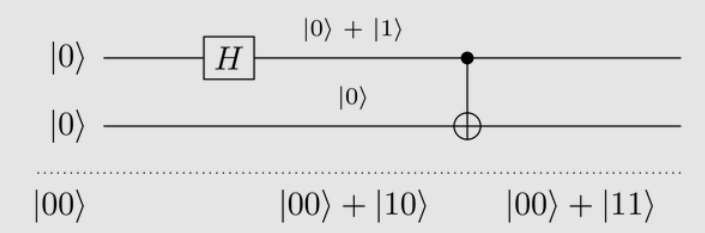
\includegraphics[width=0.6\textwidth, height=0.6\textheight, keepaspectratio]{entanglement.PNG}
  \end{center}
\end{frame}

\begin{frame}{BQP and Simulating Classical Circuits}
  \begin{itemize}
    \item Note that due to Quantum Mechanics being inherently probabilistic, we often define acceptence with respect to a certain probability. Specifically, the class $BQP$, or bounded error quantum polynomial time is the class of problems that can be solved correctly with greater than $\frac{2}{3}$ probability on quantum circuits where the size of the circuit (number of gates) is $poly(n)$. \pause
    \item Note that by simply repeating and taking majority vote a polynomial number of times, the acceptance probability can be brought arbitrarily close to $1$. This is called \emph{amplification} \pause
    \item It can further be proved that for any problem that can be solved using classical circuits, there exists quantum circuits that also solve it with $\geq \frac{2}{3}$ probability using a polynomial number of $H$ and $CCNOT$ gates relative to size of the classical circuit.
  \end{itemize}
\end{frame}

\begin{frame}{Why care about Quantum?}
  \begin{itemize}
    \item The main reason to care about Quantum computing is because it represents the most serious challenge we have yet to the \emph{Extended Church Turing Thesis}: the idea that the Turing machine not only can do anything that's physically "computable," but can do it within polynomial time of any other physically possible model of computation. \pause
    \item Most famously, Shor's algorithm is a quantum polynomial algorithm for finding a prime factorization, a well known NP problem. \pause
    \item This hints at something, either there is a very real quantum advantage that exists to the fundamental Turing machine model, which will especially be the case if we can find a quantum algorithm for NP complete problems.
  \end{itemize}
\end{frame}

\begin{frame}{Why care about Quantum?}
  \begin{itemize}
    \item Alternatively maybe factoring does have a classical polynomial algorithm, (though I personally think that's doubtful given how much time has failed to find one). \pause
    \item It could also be the case that it has quantum advantage but only for solving certain NP "intermediate" problems that factoring happens to be one of. If that's the case, then it would be helpful to study quantum computing, if not for anything then to understand the structure of what makes these problems different.
  \end{itemize}
\end{frame}

\section{Oracle Separation of NP and BQP}
% Section pages can be printed thus:
\frame{\sectionpage}

\begin{frame}{NP and BQP}
  \begin{itemize}
    \item Though they both contain P, it is unknown whether $NP \subseteq BQP$ or $BQP \subseteq NP$. \pause
    \item It is believed however that they are incomparable with respect to set inclusion - that is they each have their own respective exclusive problems. \pause
    \item Therefore their relationship is believed to look like this:
  \end{itemize}
  \begin{center}
    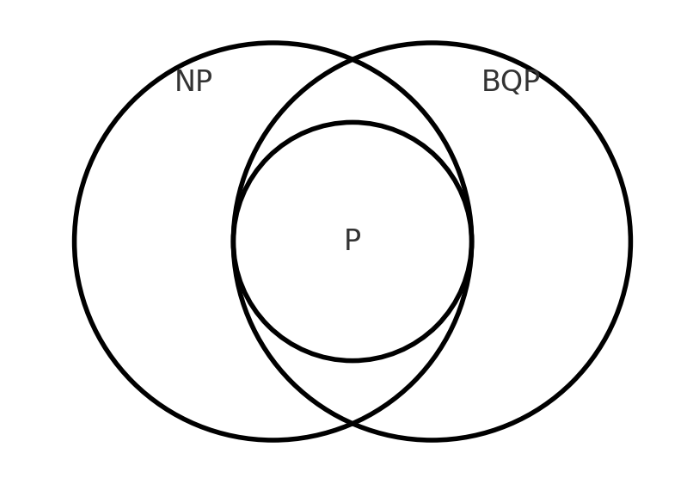
\includegraphics[width=0.5\textwidth, height=0.5\textheight, keepaspectratio]{BQP-NP.PNG}
  \end{center}
\end{frame}

\begin{frame}{Simon's Problem}
  \begin{itemize}
    \item Often the cases where quantum advantage are most exemplified are in "promise problems," problems where we're given some black box with a guaranteed promise about it's properties. \pause
    \item Simon's problem is this: given a function (and black box for it) $f: \{0, 1\}^n \rightarrow \{0, 1\}^n$ that's guaranteed to exclusively match one of two properties:
    \begin{itemize}
        \item Either injection, $f(x) = f(y) \Rightarrow x = y$
        \item Or not injective but a two-to-one Simon's function, meaning $\exists s \neq 0$ such that $\forall x, y, f(x) = f(y) \Leftrightarrow y = x \oplus s$
    \end{itemize}
    The problem is to decide which one it is.
  \end{itemize}
\end{frame}

\begin{frame}{Oracle Separations}
  \begin{itemize}
    \item Simon's theorem: $\exists$ a quantum algorithm solving this problem with $O(n)$ queries (to the given black box that computes $f$), while any classical algorithm would require $\Theta(2^{\frac{n}{2}})$ queries (the quantum algorithm later actually served as inspiration for Shor's algorithm). \pause
    \item While there is no proof that $BQP \nsubseteq NP$, we can use Simon's problem to prove there exists an oracle $O$ such that $BQP^O \nsubseteq NP^O$. \pause
    \item This is important since these \emph{oracle separations} at the very least offer heuristic evidence for the sets being different. We will proceed to show this proof.
  \end{itemize}
\end{frame}

\begin{frame}{$BQP^O$ not in $NP^O$}
  \begin{itemize}
  \item Let $\{f_n\}_{n \in \mathbb{N}}$ be a sequence of functions $f_n: \{0, 1\}^n \rightarrow \{0, 1\}^n$ such that
        \begin{align*} f_n = 
            \begin{cases}
                \text{uniform } 1-1 &\text{with probability 0.5} \\
                \text{uniform simon's function} &\text{with probability 0.5}
            \end{cases}
        \end{align*} \pause
        \item Our oracle $O: \{0, 1\}^* \rightarrow \{0, 1\}^*$ is such that on input $x$ such that $|x| = k, O(x) = f_k(x)$. \pause
        \item We will consider the language $coSimon^O = \{1^n | f_n$ is a one to one function$\}$
  \end{itemize}
\end{frame}

\begin{frame}{$BQP^O$ not in $NP^O$ Continued}
  \begin{itemize}
  \item Since Simon's theorem establishes an $O(n)$ quantum algorithm that decides Simon's problem - that is solves it for both "yes" and "no" cases with probability greater than $\frac{2}{3}$, $coSimon^O$ is clearly in $BQP^O$. \pause
  \item The reason we're considering this instead of just Simon's problem is because the secret string $s$ can be used as a certificate for an $NP$ machine to solve Simon's problem/efficiently verify any "yes" answer to a function being a Simon's function. \pause
  \item On input $1^n$ simply choose a length $n$ input $x$, compute $y = x \oplus s$ which guarantees that $x \neq y$ since $s$ is not zero, and then you'd simply verify that $O(x) = O(y)$ (which implies $f_{n}(x) = f_{n}(y)$). \pause
  \item It is not clear there is such a certificate for the "no" answers - the cases where $f_n$ is one to one, so we might hope that this can be exploited to show $coSimon^O \notin NP^O$. 
  \end{itemize}
\end{frame}

\begin{frame}{$BQP^O$ not in $NP^O$ Continued}
  \begin{itemize}
  \item The key insight is we're going to actually build the oracle $O$ and sequence $\{f_n\}_{n \in \mathbb{N}}$ that $coSimon^O$ depends on in it's definition, such that $O$ and $\{f_n\}_{n \in \mathbb{N}}$ still meet the criteria we've specified their definitions must meet. \pause
  \item However they will be constructed in such a way that $coSimon^O$ is not empty and no possible deterministic Turing machine $M$ with oracle access to $O$ can verify "yes" answers to $coSimon^O$ in polynomial time - which would prove it is not in $NP^O$. \pause
  \item This will essentially be done via a diagonal argument.
  \end{itemize}
\end{frame}

\begin{frame}{$BQP^O$ not in $NP^O$ Continued}
  \begin{itemize}
    \begin{thrm}
      $\exists O$ such that $BQP^O \nsubseteq NP^O$
    \end{thrm} \pause
    \begin{pf}
    \begin{itemize}
        \item Let $M_1, M_2,...$ be an enumeration of all Turing machines that can query some oracle (note that should we choose to replace an oracle on the same machine, it's algorithm will be the exact same - there is no difference other than the oracle's outputs and any behavior contingent on that). \pause
        \item Let $p_i(n)$ be the time $M_i$ takes which is some $poly(n)$ \pause
        \item Starting with $i = 1$, for each machine $M_i$, we choose the smallest number $n_i$ such that $f_{n_i}$ has not yet been defined and such that $p_i(n_i) \leq \sqrt{2^{n_i - 1}}$ (as that's smaller than the lower bound on number of queries needed to classically guarantee an answer for what $f_{n_i}$ is). 
    \end{itemize}
    \end{pf}
  \end{itemize}
\end{frame}

\begin{frame}{$BQP^O$ not in $NP^O$ Continued}
  \begin{itemize}
    \begin{pf}
    \begin{itemize}
        \item We choose an injective function to assign to $f_{n_i}$. For values of $n$ in between all the $n_i$'s we choose, we also choose their respective $f_n$ functions arbitrarily, however unlike the $f_{n_i}$ functions those get left alone for the rest of our construction. \pause
        \item Now we run $M_i$ on $1^{n_i}$. If the output is a "no" answer for $f_{n_i}$ being a one to one function, that is clearly incorrect and we do nothing. \pause
        \item If it's a "yes" answer, we reassign $f_{n_i}$ to be a Simon's function, but one specifically constructed so that the output of all the values in $\{0, 1\}^{n_i}$ which were queried by $M_i$ are left unchanged (remember that this is acceptable with the function still being different, since the number of possible queries is far less than total possible inputs by being less than or equal to $\sqrt{2^{n_i - 1}} < 2^{n_i}$).
    \end{itemize}
    \end{pf}
  \end{itemize}
\end{frame}

\begin{frame}{$BQP^O$ not in $NP^O$ Continued}
  \begin{itemize}
    \begin{pf}
    \begin{itemize}
        \item This implies the machine will have the exact same behavior with this function, meaning on some $NP$ certificate a "yes" will be output even though it should now be a "no" since it's a Simon's function. \pause
        \item Therefore we have guaranteed that this oracle $O$ and respective sequence we've constructed $\{f_n\}_{n \in \mathbb{N}}$ will be such that it is not possible for any $M_i$ to accept $coSimon^O$ with polynomial time verification for "yes" answers. For each one there will be some input $1^{n_i}$ that causes it to fail. \pause
        \item So $BQP^O \nsubseteq NP^O$. QED
    \end{itemize}
    \end{pf}
  \end{itemize}
\end{frame}

\begin{frame}{Final Remarks}
  \begin{itemize}
    \item There have been many oracle separations over the years in Quantum Complexity Theory, including a similar one to show $NP^O \nsubseteq BQP^O$. \pause
    \item Most significantly, in recent years it's even been found that there is an oracle separation showing $BQP^O \nsubseteq PH^O$. \pause 
    \item The implications of even these heuristic arguments for what could be actual separations are endless, and I hope like me you see how it's an exciting time for the field!
  \end{itemize}
\end{frame}

\begin{frame}{The End}
  \begin{itemize}
    \item "Turning to quantum mechanics...secret, secret, close the doors! we always have had a great deal of difficulty in understanding the world view that quantum mechanics represents... It has not yet become obvious to me that there’s no real problem. I cannot define the real problem, therefore I suspect there’s no real problem, but I’m not sure there’s no real problem. So that’s why I like to investigate things." - Richard Feynman 
    \item Classes to take if you love this stuff: CS 474, CS 475, CS 579, special topics CS quantum computing and quantum complexity offerings.
  \end{itemize}
\end{frame}

\end{document}